\begin{frame}{意味のある「統計」期間について}{検証}
  \lead{上空の対流圏の風は、時期を知ってもほとんど当てられない}
  \begin{columns}[T]
    \begin{column}{0.56\textwidth}
      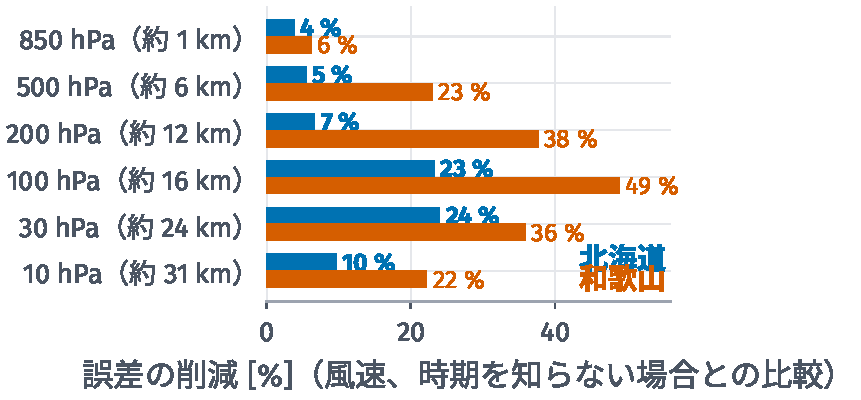
\includegraphics[width=\linewidth,height=126pt,keepaspectratio]{S_level_skill_both.pdf}
    \end{column}
    \begin{column}{0.42\textwidth}
      \begin{itemize}\itemsep 1.5mm
        \item \kw{地上付近は 4--6 \%}\\地上風は当日の予報で判断する
        \item \kw{北海道の 200 hPa は 7 \%}\\ジェットの高さでも暦は効かない
        \item 役に立つのは \kw{16--24 km}\\（100--30 hPa の帯）
      \end{itemize}
    \end{column}
  \end{columns}
  \srcline{風速の 1 年抜き交差検証、最良ビン幅でのスキル}
\end{frame}
